%%%%%%%%%%%%%%%%%%%%%%%%%%%%%%%%%%%%%%%%%
% Stylish Article
% LaTeX Template
% Version 2.1 (1/10/15)
%
% This template has been downloaded from:
% http://www.LaTeXTemplates.com
%
% Original author:
% Mathias Legrand (legrand.mathias@gmail.com) 
% With extensive modifications by:
% Vel (vel@latextemplates.com)
%
% License:
% CC BY-NC-SA 3.0 (http://creativecommons.org/licenses/by-nc-sa/3.0/)
%
%%%%%%%%%%%%%%%%%%%%%%%%%%%%%%%%%%%%%%%%%

%----------------------------------------------------------------------------------------
%	PACKAGES AND OTHER DOCUMENT CONFIGURATIONS
\usepackage{placeins}
\usepackage{float}
%----------------------------------------------------------------------------------------

\documentclass[fleqn,10pt]{SelfArx} % Document font size and equations flushed left

\usepackage[english]{babel} % Specify a different language here - english by default

\usepackage{lipsum} % Required to insert dummy text. To be removed otherwise

%----------------------------------------------------------------------------------------
%	COLUMNS
%----------------------------------------------------------------------------------------

\setlength{\columnsep}{0.55cm} % Distance between the two columns of text
\setlength{\fboxrule}{0.75pt} % Width of the border around the abstract

%----------------------------------------------------------------------------------------
%	COLORS
%----------------------------------------------------------------------------------------

\definecolor{color1}{RGB}{0,0,90} % Color of the article title and sections
\definecolor{color2}{RGB}{0,20,20} % Color of the boxes behind the abstract and headings

%----------------------------------------------------------------------------------------
%	HYPERLINKS
%----------------------------------------------------------------------------------------

\usepackage{hyperref} % Required for hyperlinks
\hypersetup{hidelinks,colorlinks,breaklinks=true,urlcolor=color2,citecolor=color1,linkcolor=color1,bookmarksopen=false,pdftitle={Title},pdfauthor={Author}}

%----------------------------------------------------------------------------------------
%	ARTICLE INFORMATION
%----------------------------------------------------------------------------------------

\JournalInfo{Text Mining \& Search Project} % Journal information
\Archive{A.Y. 2019-2020} % Additional notes (e.g. copyright, DOI, review/research article)

\PaperTitle{Methodological approaches for Text Summarization} % Article title

\Authors{\textbf{Riccardo Cervero}, \textbf{794126}\textsuperscript{*}} % Authors
\affiliation{\textsuperscript{*}\textit{Universita` degli Studi di Milano Bicocca, CdLM in Data Science}} 

\Keywords{Abstractive Summarization --- Extractive Summarization} % Keywords - if you don't want any simply remove all the text between the curly brackets
\newcommand{\keywordname}{Keywords} % Defines the keywords heading name

%----------------------------------------------------------------------------------------
%	ABSTRACT
%----------------------------------------------------------------------------------------

\Abstract{Customer reviews can often be long and descriptive. Analyzing these reviews manually, as you can imagine, is really time-consuming. This is where the brilliance of Natural Language Processing can be applied to generate a summary for long reviews. We will be working on a really cool dataset. Our objective here is to generate a summary for the Amazon Fine Food reviews using the abstraction-based approach we learned about above.}

%----------------------------------------------------------------------------------------

\begin{document}

\flushbottom % Makes all text pages the same height

\maketitle % Print the title and abstract box

\tableofcontents % Print the contents section

\thispagestyle{empty} % Removes page numbering from the first page

%----------------------------------------------------------------------------------------
%	ARTICLE CONTENTS
%----------------------------------------------------------------------------------------

\section{Dataset Exploration} 
The texts to be summarized hails from a portion of the \href{https://www.kaggle.com/snap/amazon-fine-food-reviews}{"Fine Food Reviews"} dataset, recording 100,000 natural-language-written reviews in English from more than 70,000 Amazon users. The original data span from October 1999 up to October 2012, including, besides plain text reviews, product and user information, ratings and, above all, a very brew reference summary offered by database providers which will constitute the ground truth during the neural network training phase and an evaluation benchmark.\\
As seen from the plot, ratings distribution is heavily unbalanced towards most positive score.
\par
{\centering\vspace{10pt}
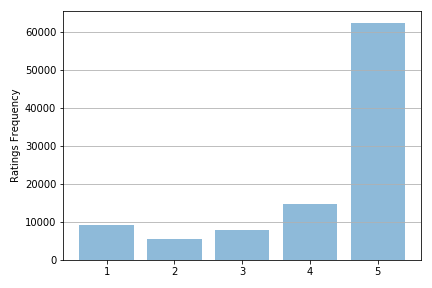
\includegraphics[width=8cm, height=5cm]{r_dist.png}
\captionof{figure}{Ratings distribution\label{fig:img1}}
\vspace{10pt}
\par}
As far as reviews, the average number of sentences is 5, while about one sentence on average is used to summarize the content. The number of sentences in the original document can affect extractive results of summarization, and its distribution shows, in the first case, a slight concentration around the mean\footnote{Reviews composed by a number of sentences between 3 and 7 are about 64\% of the total.}, with a very long and thin tail.\par
{\centering\vspace{10pt}
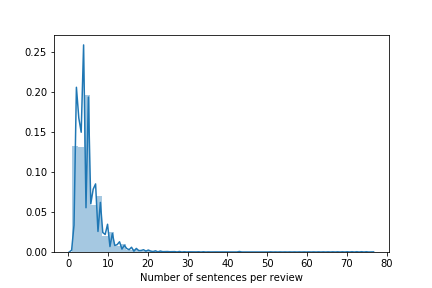
\includegraphics[width=9cm, height=5cm]{text_dist.png}
\captionof{figure}{Distribution of number of sentence per review\label{fig:img1}}
\vspace{10pt}
\par}
Nevertheless, even though this characteristic of homogeneity could help avoid bias during generation and comparison of several summaries, it is counterbalanced by a greater variability\footnote{While coefficient of variance for sentences count is about 74\%, the one related to word count is 102\%} in the number of words per review.
\par
{\centering\vspace{10pt}
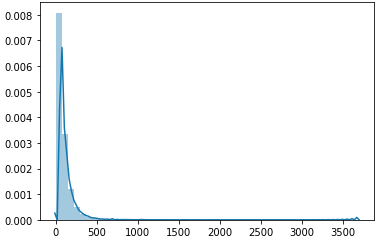
\includegraphics[width=8.2cm, height=4.2cm]{word_dist.png}
\captionof{figure}{Distribution of number of word per review\label{fig:img1}}
\vspace{10pt}
\par}
Finally, it is possible to get a first insight on vocabulary composition by representing the corpus \textit{wordcloud}. 
\par
{\centering\vspace{10pt}
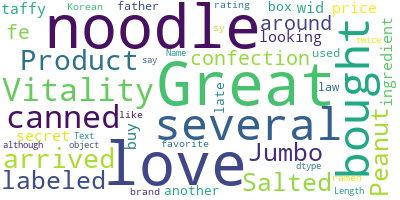
\includegraphics[width=8.2cm, height=4.2cm]{wc.png}
\captionof{figure}{Corpus WordCloud\label{fig:img1}}
\vspace{10pt}
\par}
%------------------------------------------------
\section{Text Pre-processing}
Review is a particular kind of text, often composed by neither non-professional writer nor journalist which thus tends to resemble spoken language, because includes abbreviations, slang and informal phrases, errors in punctuation and misspellings, etc. This documents appear as a mixture of heterogeneous forms of text, even presenting different lexical and syntactic structures within the same document. For this reason, pre-processing operations are compulsory to help reduce distortion and try to convert the corpus into standard form. This goal is achieved in a preliminary way through the following operations. After having tokenized\footnote{Separator character used is \textit{white-space}.} the document, as text normalization phase, it is necessary to convert all informal expressions that occur in form of contractions\footnote{Such as \textit{couldn't}, which should be replaced by \textit{could not}} and put all the tokens to lower case. The second step consist in removing noisy part of the text to be analyzed: genitives, punctuation, symbols, special characters and numbers. Finally, stop words are eliminated because this very frequent tokens are useless and could distort the co-occurrence analysis during the stage of text representation. Neither stemming nor lematization operations are performed, because inflected and derived tokens provide fundamental information that both simplest algorithms and neural network cannot afford to lose during elaboration of a summary containing the most relevant concepts.\\
In each following methodology, the aforementioned operations will be applied separately to each sentence extracted from the text by means of a \textit{sentence tokenizer}, so as to return a list of \textit{cleaned} sentences. The \textit{sentence tokenizer} uses an unsupervised algorithm to build a model for detecting sentence boundaries\footnote{Algorithm is called \href{https://www.nltk.org/_modules/nltk/tokenize/punkt.html}{\texttt{PunktSentenceTokenizer}}.}, which has proven to be an effective approach for many European languages.
%------------------------------------------------
\section{Extractive Summarization}
Extractive summarization aims to recognize most important sections of a text to generate a subset of the sentences. Between the two approaches, this is certainly the most superficial, as it returns a simple verbatim reduction of the original document.
\subsection{Topic representation methods}
These methods generate an intermediate representation capturing discussed topics and score each sentence according to its importance. This class includes methods that vary mainly on the basis of the intermediate representation that they are able to extract. One of them is the matrix factorization based Latent Semantic Analysis.
\subsubsection{Latent Semantic Analysis}
Latent Semantic Analysis (\textit{LSA}) is an unsupervised technique extracting an implicit representation of semantics within text identifies several. It identifies several patterns of co-occurring words as weighted relevant topics, without using lexical resources. Based on distributional hypothesis, assumes that words close in meaning will occur in similar location of text, thus, in case of text summarization, in same sentences. In this way, it is possible to understand which sentence deals with which topic and to select sentences related to most important themes.
The algorithm is implemented with following steps. Topics representation starts with filling an $nxm$ matrix $A$, each row corresponding to an input word and each column to a sentence. Each entry $a_{ij}$ records the weight of the i-th word in the j-th sentence, zero if the word is not contained in the sentence. Non-zero values can be of three types:
\begin{itemize}
  \item Term Frequency $tf_{t,s}$, which is not convenient because does not consider the different number of words within a sentence. In fact, it is better that weights of words from a short sentence are bigger, as we can say they exerts more influence;
  \item Term Frequency normalized by sentence length $\frac{tf_{t,s}}{|s|}$
  \item Tf-idf $$tf.idf=\frac{tf_{t,s}}{|s|}\bullet log(\frac{N}{df_t})$$ which derives from the product between $tf$ and \textit{inverse document frequency} $idf$. This value proportionally measures both frequency in the single sentence and the diffusion in the other ones, thus increasing with the rarity of the term in the collection, that is the specificity of that term in relation to that sentence. For this reason, it is the most correct weighting function for this type of co-occurence analysis.  
\end{itemize}
Matrix $A$ can be decomposed into three sub-matrices:
$$A=U\Sigma V^T$$
where:
\begin{itemize}
    \item $U$ records the weight of each word for each topic
    \item $\Sigma$ is a diagonal matrix whose non-zero values represent topic importance
    \item $V^T$ consists of a new representation of the sentences, each expressed no longer in terms of the words it contains but in terms of the topics it relates to:
\end{itemize}
The product $D=\Sigma V^T$ combines topic importance scores with the new representation of the sentences and indicates to what extent the sentence communicates a certain topic. Therefore, $d_{ij}$ is the weight of the argument i for the sentence j.\\
Sentences presenting many of the most important topics - based on weights recorded in $\Sigma$ matrix - are often excellent candidates for the summary. For this reason, the algorithm identifies these candidates by calculating for each sentence  $$s_i=\sqrt{\sum_{j=1}^md^2_{ij}}$$
\\
As anticipated, when the algorithm uses the term frequency divided by the length, it tends to favor shorter sentences with frequent terms, while exploiting tf.idf function it operates an additional filter on those sentences that contain rarer words, those more "specialized" with respect to the topic. On the contrary, application of simple term frequency weights only makes method focus on the raw number of times a word occurs.
\subsection{Indicator Representation methods}
Original text can also be analyzed by means of a set of relevance indicators, which do not aim to discover topics. In this case, each sentence is indeed described by a list of features - such as length of the sentence, position in the document, presence of certain words, etc -, which can be then combined in many ways to obtain a unique scoring useful to rank and select most important sentences. Three different approaches have been implemented.
\subsubsection{Graph-based: TextRank}
Graph-based summarization methodologies derive from PageRank algorithm, which assigns numerical weights to the related elements of a set, with the aim of quantifying the relative importance within the group. In this case, the method will represent the entire review as a network of inter-connected sentences, each one associated with a node. Edges join these vertices if and only if the similarity between the two given sentences exceeds a certain threshold. At the end, graph representation will return two outputs:
\begin{itemize}
    \item the graph partition from which it is possible to deduce a set of discrete topics extracted from the corpus 
    \item important sentences, namely those connected with many of the others in the partition, and which will most likely be included in the summary
\end{itemize}
Among all the existing variants, the most popular was chosen: the \textit{TextRank} algorithm. First of all, \textit{TextRank} splits the review into sentences - with the aforementioned \textit{sentence tokenizer} - and applies pre-processing operations to them.\\
Then, a vector representation for every sentence has to be produced. An alternative would be to resort to the weighting functions used with \textit{LSA}, but using them to measure similarity would bring a strong limitation, because they do not take into account syntactic and semantic information, like the order of the words. For this reason, sentences will be represented through the word embeddings produced by the pre-trained model called \textit{"Global Vectors for Word Representation"} \textit{GloVe}. GloVe is an unsupervised learning algorithm for obtaining words vector representations\footnote{Precisely, we will be using the pre-trained \textit{Wikipedia 2014 + Gigaword 5 GloVe} vectors}. This embeddings are created by mapping words into a space where the distances are related to semantic similarity. Training is performed by extracting global statistical information from the non-zero values of a co-occurence word-word matrix, rather than 
from the entire sparse matrix - like matrix factorization methods do - or from the single context window within the large corpus, - like \textit{word2vec} does. The resulting representations show interesting linear substructures of the word vector space.\\
\textit{GloVe} will thus consider 400k terms\footnote{If otherwise embedding of one word does not exist, the algorithm returns a vector of zeros.}, each one described by an array of 100 values. Finally, sentences vector representation will be obtained by computing the mean of all the vectors representing each word in the given sentence, gaining a consolidated vector for the sentence.\\
The third step consists in compute the cosine similarity among all the sentence vectors and store it into a $nxn$ matrix.\\
This similarity matrix is converted into a graph, with sentences as vertices and similarity scores as edges.\\
Hereafter, \textit{TextRank} implements \textit{PageRank} algorithm to extract an importance score, as aforementioned, and rank sentences based on their score. Finally, the final summary is created by selecting the top N sentences.
\subsubsection{TextRank variant}
This project also calls for the implementation of a packaged TextRank variant: \texttt{PytextRank}. This performs a lemmatization of the text, constructing a \textit{lemma graph} to represent links among the candidate sentences.
\subsubsection{Feature-based: Luhn's Algorithm}
Luhn's Algorithm is an early heuristic method which performs extractive summarization task by computing the “significance” of the word from the frequency. The significance in the document is interpreted as an evaluation of the relevance of a term within the sentence. The algorithm is a naive approach based on $tf$ representation and looking at the “window size” of non-important words among relevant words.\\
The stages are:
\begin{enumerate}
  \item Extraction of keywords in the text, namely signficant terms, by selecting those above a mininum threshold of - normalized by review length - term frequency $\frac{tf_{t,d}}{|d|}$ and under a maximum, thus ignoring most frequent and rare ones 
  \item Computation of sentences weights based on the squared number of keywords divided by the windows size, which is the maximum distance between two significant words: $$s_i=\frac{\text{Number}^2\;\text{of Keywords in i}}{\text{Span}}$$
  \item Sorting sentences in descending order of score and selection of the best N-ranked.
\end{enumerate}
In this case, minimum and maximum are chosen to be respectively 5\% and 50\%.\\
To sum up, the most important sentence will be the one maximizing the number of terms which are neither too frequent - over the half number of tokens in the entire review - nor too rare and/or minimizing the span between most distant keywords.
\subsubsection{Deep Learning based: BERT Summarizer}
All summarization models just presented have big limitations. Beyond technical reasons, this is due to the existence of a semantic threshold dividing the human being from the computer: men, in fact, manage to recognize the context of the sentences at a greater depth, extracting more clear meanings. Although it could not be enough to break down this threshold, to obtain better summaries it is necessary to reach a higher level of abstraction in the model, able to capture as much information as possible from the text. For this reason, neural networks are used. In particular, one of the neural networks most frequently involved in natural language processing tasks is BERT model.\\
\textit{Bidirectional Encoder Representations from Transformers BERT} is a pre-train deep bidirectional neural network which offers representations from unlabeled text. While directional models read text sequentially - left-to-right or right-to-left -, BERT reads the entire sequence of words at once. This characteristic allows it to learn the context of a word based on all of its surroundings: both left and right words. In details, the context is extracted by a Transformer, an attention mechanism that finds contextual relations between terms in a text. Thus Transformer includes two separate components:
\begin{itemize}
    \item an encoder reading input review
    \item a decoder producing a prediction for the NLP task to be accomplished. 
\end{itemize}
For any of these tasks, BERT's goal is to generate a language model, represented by a sequence of vectors in output, each one associated to an input token.\\
Moreover, the analysis is enhanced by using \textit{coreference techniques}. \textit{Coreference} occurs when two or more expressions in a text refer to the same entity. In computational linguistics, to derive the correct interpretation of a text and estimate the relative importance of various mentioned subjects, referring expressions must be connected to the right element. In this way, BERT succeeds in inferring a better context for each word.\\
As said, this neural network can be modified to create several state-of-art models for NLP tasks. In particular, as far as text summarization, a \textit{Bert Extractive Summarizer} has been recently released by fine-tuning BERT architecture. This Summarizer works by first embedding the single tokens. Secondly, it builds a "Segmentation Embedding" to detect sentences boundary and embed them. Thirdly, the model embeds position in the document. Finally, the algorithm performs a clustering process, finding the sentences that are closest to the cluster's centroids.
\par
{\centering\vspace{10pt}
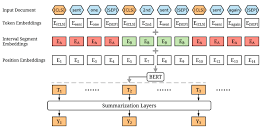
\includegraphics[width=8.2cm, height=4.2cm]{BERT.png}
\captionof{figure}{Text Representation in BERT Summarizer\label{fig:img1}}
\vspace{10pt}
\par}
%------------------------------------------------
\section{Abstractive Summarization}
Differently from what has been done up to now, abstractive summarization is not configured as a mere selection of important sentences - based on completely different criteria - but as a method to express the concepts of the source in a new interesting form. The model learns and reproduces its own expressions and sentences to offer a more coherent summary, similar to what a human being would generate. In this way, its result will not copy the original structure, words and sub-sentences - the majority of which, even if present in the most relevant sentence, often prove to be useless. On the contrary, the information needed to achieve the goal will be searched in the patterns contained within a training corpus.It is therefore clear how, in this case, it is fundamental to implement an even more complex model than the previous one.
\subsection{Seq2Seq Modeling with Attention Mechanism}
A "\textit{Sequence-to-Sequence}" task is a problem involving sequential information. Text Summarization can be considered as a sequence modelling problem, because any prediction depends on the analysis of the sequence of tokens and sentences. More precisely, it is configured as a \textit{Many-to-Many Seq2Seq} problem, where both input and output - the original Amazon reviews and respective summaries - are sequences composed by more than one token.\\
As explained in the previous section, the typical \textit{Seq2Seq} model relies on two principal components: an encoder and a decoder. The task of the encoder network is to create a smaller dimensional representation of the input text. This representation is then forwarded to a decoder network which generates a sequence of its own that represents the output. This \textit{encoder-decoder} architecture is particularly suitable, as is the case with Text Summarization, when input and output sequences are of different lengths.\\
The preferred class of models for such operations is therefore that of \textit{Recurrent Neural Networks (RNNs)}. What distinguishes \textit{RNNs} from normal feed-forward networks is that hidden layers, in addition to inputs from the input layer, also receive their own output associated with the previous state, conveniently weighted. This mechanism serves to provide the neural network with a memory about the sequence of tokens. Nevertheless, \textit{RNNs} are not able to model long-term dependencies because their back propagation algorithm can cause two negative effects: vanishing gradients and exploding gradients. For this reason, other models are preferred that can avoid these risks and describe the dependencies among tokens within long documents. In this project, the chosen alternative is \textit{Long Short Term Memory LSTM}, wherein the function just mentioned is implemented through blocks - gates -, executing several operations.\\ Thus, the final architecture is constituted by two neural networks: an \textit{Encoder LSTM} and a \textit{Decoder LSTM}.
\subsubsection{Training}
During this stage, encoder and decoder work together to learn the best way to predict the target sequence.\\ At each timestep, the Encoder receives an additional word of the sequence, processes the new data and acquires the contextual information. Then, the final state of the Encoder, i.e. the output of the last timestep, initializes the Decoder component, which in turn reads the entire target sequence token-by-token and predicts a sequence offset at each timestep. In this way, the Decoder \textit{LSTM} is trained to predict the next word in the sequence given the previous one.\\
\textit{"start"} and \textit{"end"} in Figure 6 are special tokens added to the target sequence before passing it to the Decoder which respectively begin and stop the prediction.\par
{\centering\vspace{10pt}
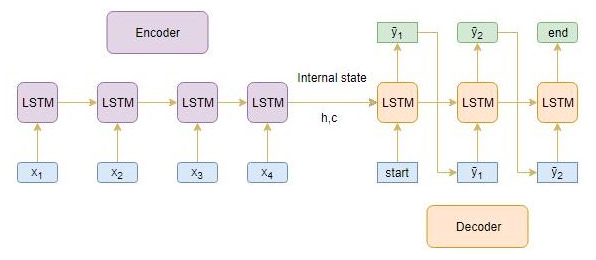
\includegraphics[width=8.2cm, height=4cm]{LSTM.png}
\captionof{figure}{Encoder-Decoder LSTM architecture\label{fig:img1}}
\vspace{10pt}
\par}
\subsubsection{Inference}
After training, the model is tested on new reviews whose target sequence is unknown. Inference process involves 6 steps:
\begin{enumerate}
    \item Encoding of the input sequence and initialization of Decoder with subsequent internal states of the Encoder
    \item Passing of \textit{"start"} token as input to the Decoder
    \item Running of the Decoder in combination with the internal states related to current timestep 
    \item Computation of the probability for the next word and selection of the one maximizing this probability
    \item Passing of this selected word as an input to the Decoder in the next timestep and update the internal states with the current timestep
    \item Repetition of 3rd, 4th and 5th step until
    \begin{itemize}
        \item \textit{"end"} token is generated, i.e. when the input sequence runs out
        \item[] \textbf{or}
        \item when hitting a maximum target sequence length 
    \end{itemize}
\end{enumerate}
\subsubsection{Attention Mechanism}
This architecture composed of an Encoder, which converts input into fixed length vectors, and Decoder, which predicts summaries by reading this entire embedding, is plagued by a main limitation: the Encoder struggles to compress long input sentences into a vector and the performance of the neural network deteriorates rapidly as the length increases. This bottleneck is overcome thanks to the so-called \textit{"Attention Mechanism"}, which aims to produce the next word by looking only at specific parts of the sequence. The key intuition behind it consists in selecting the words of the input text which are more relevant to generate a new token at each timestep. First, this is made by computing a score $e_{ij}$ evaluating the alignment between
\begin{itemize}
    \item $h_j$, i.e. the hidden state output by Encoder at each timestep of the input sequence j
    \item $s_i$, i.e. the hidden state output by Decoder at each timestep of the target sequence i 
\end{itemize}
In other words, $e_{ij}$ is based on semantic links among input and target tokens, and, in our case, corresponds to the following additive formulation:
$$e_{ij}=V^Ttahn(W[s_i,h_j])$$ 
where $V$ and $W$ are the two trainable weights matrices for the neural networks, thanks to which it learns to predict the next word in the sequence. The $e_{ij}$ scores are converted to mutually exclusive probabilities using a softmax function, producing the so-called "attention weights": 
$$a_{ij}=\frac{e^{e_ij}}{\sum_{k=1}e^{e_ik}}$$
Then, computing the linear combination among the attention weights and hidden states of the decoder $h_j$, the algorithm extract the context vector of timestep i $C_i$. $C_i$ is concatenated to the hidden state of the decoder at timestep i $s_i$, and this result is finally mapped to the output: the word at timestep i, $\hat{y}_i$ in Figure 6.\\
\subsubsection{Final model}
SONO DUE RETI
Stacked LSTM: it is composed of 3 LSTM 

SPIEGA 'rmsprop' E loss='sparse\_categorical\_crossentropy'\\

The final model architecture appears as in the Figure 7.
\par
{\centering\vspace{10pt}
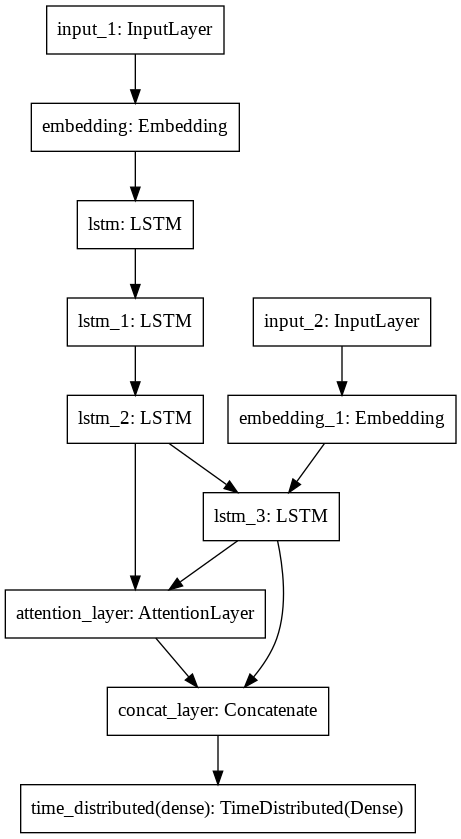
\includegraphics[width=8.2cm, height=11cm]{model.png}
\captionof{figure}{Final model architecture\label{fig:img1}}
\vspace{10pt}
\par}
Due to the early stopping condition, the model training stopped at 29th epoch, requiring almost 7 hours. The learning process is visualized with Figure 8:
\par
{\centering\vspace{10pt}
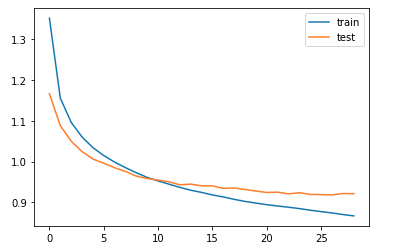
\includegraphics[width=8cm, height=5cm]{vizproc.png}
\captionof{figure}{Loss results over the epochs\label{fig:img1}}
\vspace{10pt}
\par}
A slight increase in the validation loss is shown after tenth epoch.
%------------------------------------------------
\section{Evaluation}
Only one sentence
%------------------------------------------------
\section{Results and Discussion}
%----------------------------------------------------------------------------------------
%	Code
%----------------------------------------------------------------------------------------
\section*{Code}
\href{https://github.com/RCrvro/Text-Summarization-Project}{Code is available at this link.}
%----------------------------------------------------------------------------------------
%	REFERENCE LIST

%----------------------------------------------------------------------------------------
\phantomsection
\bibliographystyle{unsrt}
\bibliography{sample}
GloVe: https://nlp.stanford.edu/projects/glove/

PyTextRank: https://pypi.org/project/pytextrank/

Luhn: http://courses.ischool.berkeley.edu/i256/f06/papers/luhn58.pdf

BERT: https://arxiv.org/abs/1810.04805

BERT Architecture: https://towardsdatascience.com/bert-explained-state-of-the-art-language-model-for-nlp-f8b21a9b6270

Bert Extractive Summarizer: https://pypi.org/project/bert-extractive-summarizer/

BEAM SEARCH: https://www.analyticsvidhya.com/blog/2018/03/essentials-of-deep-learning-sequence-to-sequence-modelling-with-attention-part-i/?utm_source=blog&utm_medium=comprehensive-guide-text-summarization-using-deep-learning-python 

Bahdanau Attention: https://arxiv.org/pdf/1409.0473.pdf
%----------------------------------------------------------------------------------------

\end{document}
